\documentclass[12pt]{article}
\usepackage[utf8]{inputenc}      % For UTF-8 support
\usepackage[T1]{fontenc}
\usepackage{lmodern}
\usepackage{geometry}
\usepackage{booktabs}            % For nicer tables
\usepackage{hyperref}            % For hyperlinks in the document
\usepackage{graphicx}            % For images
\usepackage{array}               % For extended table features
\usepackage{setspace}
\usepackage{csquotes}
\usepackage[backend=biber, style=ieee]{biblatex}
\addbibresource{bibliography.bib}
% \usepackage{xcolor}
% \pagecolor{gray}      % Set background color to black
% \color{white}          % Change text color to white
\usepackage{helvet}
\renewcommand{\familydefault}{\sfdefault}
\geometry{margin=1in}
\setstretch{1.15}
% \title{This is Main title \\ [0.2em]\large This is Subtitle}
% \title{Used Car Characteristics \\ [0.2em]\large An Explanatory Data Analysis}
% \author{Dávid Fodor \and Faisal Zayeem Ahmed \and Márió Palágyi}
% \date{Submission date: TBD}

\begin{document}

\begin{titlepage}
  \centering
  \vspace*{1in}
  {\Huge\bfseries Used Car Characteristics\par}
  \vspace{0.5em}
  {\Large An Explanatory Data Analysis\par}
  \vspace{1.5in}
  {\Large Dávid Fodor \\ Faisal Zayeem Ahmed \\ Márió Palágyi\par}
  \vfill
  {\large Submission date: TBD\par}
  \vspace{0.5in}
  {\large Datascience Capstone Project - IMC Krems}  % Optional: use the current date
\end{titlepage}

\section*{Abstract}
A brief overview of the project, including problem statement, methodology, key findings, and conclusions.

\section{Introduction}
\textbf{Problem Statement:} Describe the problem.\\[1ex]
\textbf{Objectives:} List the objectives and tasks required to be completed.\\[1ex]
\textbf{Data:} Describe your dataset.\\[1ex]
\textbf{Background Information:} Provide context and challenges based on your understanding of the problem.

\section{Literature Review}
Summary of relevant research and related works in the field. This section does not need to be exhaustive; include background knowledge on how the problem has been addressed before and how you plan to solve it.

Luckily, there is plenty of literature on the topic of used car prices, particularly the prediction seems to be a popular topic. Searching on Google Scholar for "used car price prediction" yields almost a million results.

\begin{figure}[ht]
  \centering
  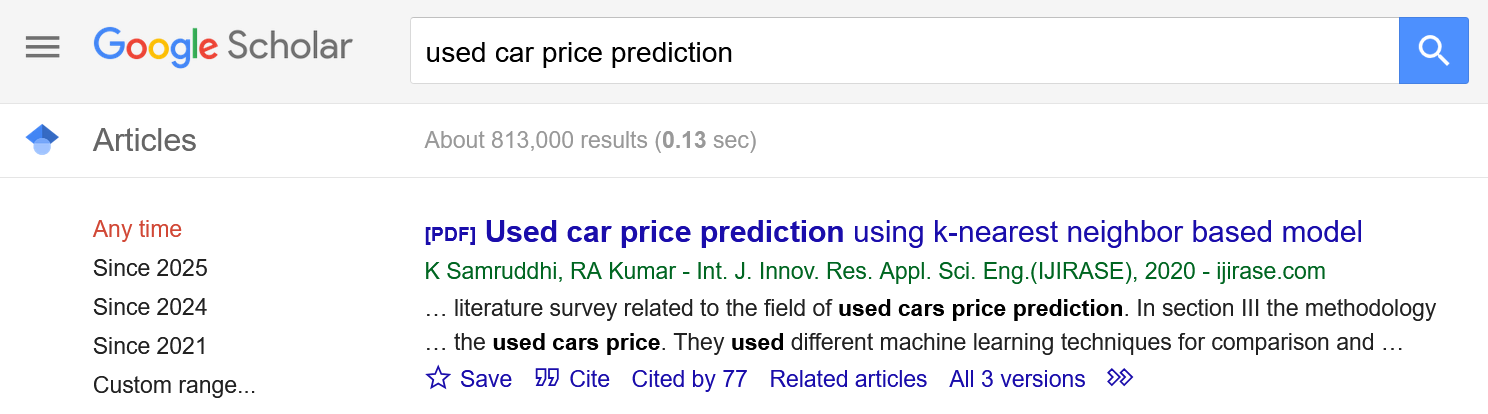
\includegraphics[width=0.8\textwidth]{./images/google_scholar.png}
  \caption{Screenshot of Google Scholar Search. Source: Google Scholar}
  \label{fig:google_scholar}
\end{figure}

However, looking for papers that solely try and explore the data and find interesting patterns is lot more difficult. Mostly, the exploration of all the data is done in the context of a prediction model, which is why we also aim to create a usable prediction model as part of our assignment.

Here, as the literature review is a small portion of the report, I will just mention some of the interesting conclusions we have found from others. Firstly, there is seemingly no real consensus on what the best model is for predicting car prices. The the data is usually scraped by the authors \cite{gegicCarPricePrediction2019}\cite{bukvicPricePredictionClassification2022}\cite{jinPricePredictionUsed2021}, or taken from a source like Kaggle \cite{zhengMachineLearningOptimization2025}\cite{nandanPreownedCarPrice2023}.

Most of the papers that compared multiple models, found that more complex models, such as \textbf{XGBoost} \cite{nandanPreownedCarPrice2023}, \textbf{Random Forest} \cite{vossResalePricePrediction}\cite{jinPricePredictionUsed2021} or \textbf{Neural Netwroks}\cite{liuResearchPredictionModel2022} worked the best, but the differences were often not so significant, the best models achieved were usually between \textit{85-95\%} accuracy.
There were some surprises too, some have found that rather interestingly other methods worked better for them, such as \textbf{SVM} \cite{shaprapawadCarPricePrediction2023a}, \textbf{LightGBM} \cite{liResearchUsedCar2022} or \textbf{Linear Regression} \cite{bukvicPricePredictionClassification2022} in case of a smaller dataset.

Some other interesting findings include for example Zheng Y. \cite{zhengMachineLearningOptimization2025} for whom the most challenging part of price prediction in his case of XGBoost, Random Forest and Linear Regression was of predicting the price of premium cars, the models constantly underestimated them, leading to worse accuracy. The author also suggests taking extra special care when cleaning outliers in price. 
Chen et al. \cite{chenComparativeAnalysisUsed2017} split their dataset into three distinct groups, once using just cars of the same make and build year, once just a car series and once all data together. They found that random forest worked all round better than linear regression, and that the more records and more features they included, the greater this distance became. This and other papers also suggest that we should not bother with linear regression in cases of larger, more complex datasets.
Nandan et al. \cite{nandanPreownedCarPrice2023} had a similar experience to us with their large amount of missing values and they also had features reminescent of ours in their Kaggle dataset, they solved the missing values issue with the following method, which they found most optimal and we shall also try to implement in our case:

\begin{displayquote}
  "To replenish the missing values in the data, the IterativeImputer technique is employed, with a variety of estimators being developed and their respective MSEs being generated ... the ExtraTreesRegressor estimator is preferable for the imputation strategy in the case of missing value"
\end{displayquote}

Huang et al. \cite{huangUsedCarPrice2022} had similarly many features to us, leading them to use a forward feature selection which we also plan on implementing due to the large number of features we have. One more interesting thing to note is how they came up with their final prediction, which is a weighted average of their different already well functioning models.

\begin{displayquote}
  "...weighted average fusion of XGBoost, CatBoost, LightGBM, and ANN. Its R2 can reach 0.9845, and the prediction effect is the best."
\end{displayquote}

\begin{figure}[ht]
  \centering
  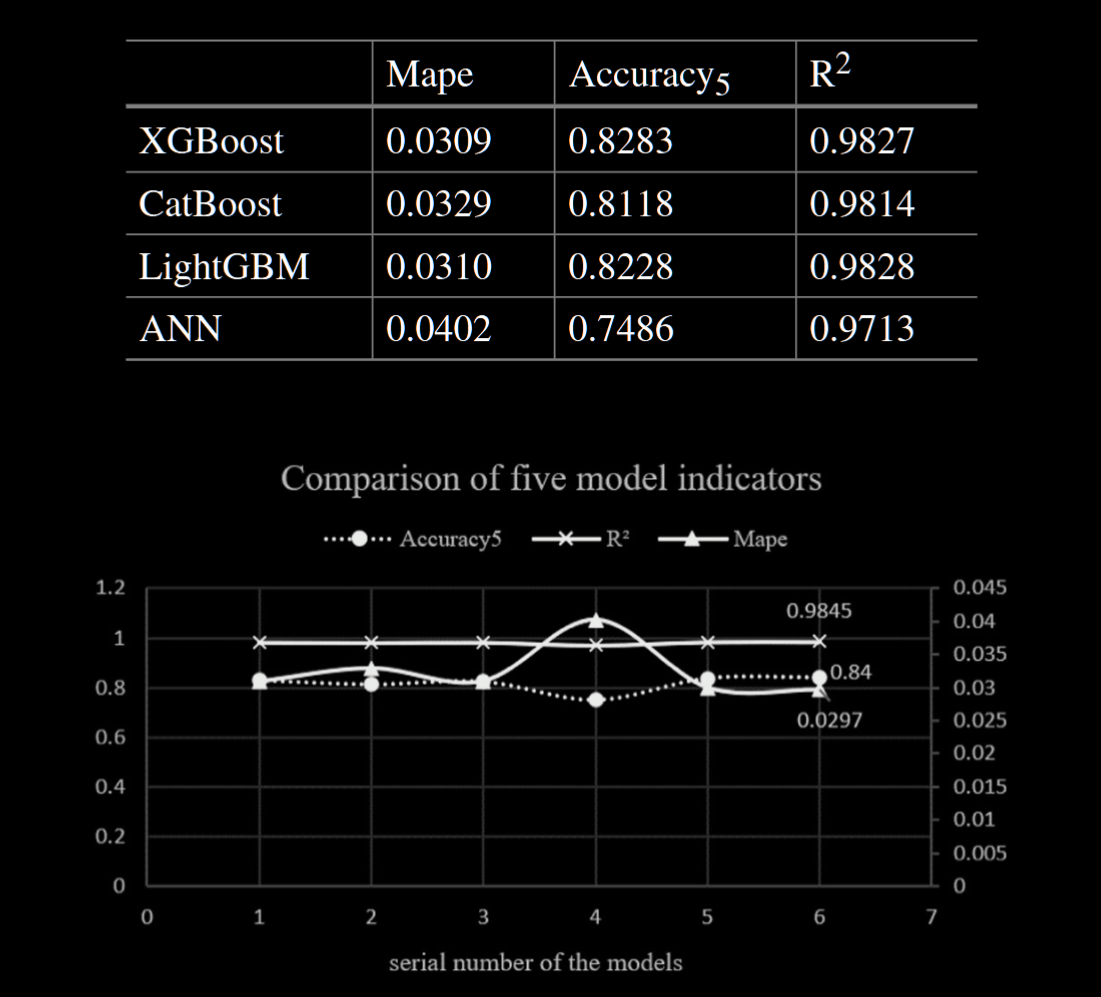
\includegraphics[width=0.8\textwidth]{./images/huang_et_al_findings.png}
  \caption{Huang et al. comparative performance of models. Source: \cite{huangUsedCarPrice2022}}
  \label{fig:huang_et_al_findings}
\end{figure}

As a conclusion of the literature review, we can safely say that there is no real consensus on what the best model may be for predicting car prices, which may be due to many factors, like the different datasets, different preoprocessing steps and different features. However, we can also see that the more complex models perform better in exploring more nuanced relationships, leading to better predictions as corroborated by Voß S. \cite{vossResalePricePrediction}. Models such as XGBoost and Random Forest seem to be some of the most popular ones, and they are also the ones that we will be expecting to work the best for our case.

\section{Methodology}

\begin{itemize}
    \item \textbf{Data Collection, Description and Management:} Describe the steps involved in data collection or preprocessing, including EDA.
    \item \textbf{Analysis Techniques:} Describe your approach to solving the problem. You can include a model diagram to illustrate your method.
    \item \textbf{Tools and Software Used:} List the tools, frameworks, and software used for the project.
\end{itemize}

\subsection{Data Collection}

In our case the data collection is a rather interesting part of the project, which took quite some time. Unlike other groups, we had to find our own primary datasource, seeking a used car marketplace which we could scrape.
After several trials of scraping different websites, we finally ended up with one that was quite lenient with their robots.txt file, and we could scrape it without any issues. The website we used was \url{https://www.autoscout24.com/}, which is one of the largest used car marketplaces in Europe boasting more than 2 million listings.

\begin{figure}[ht]
  \centering
  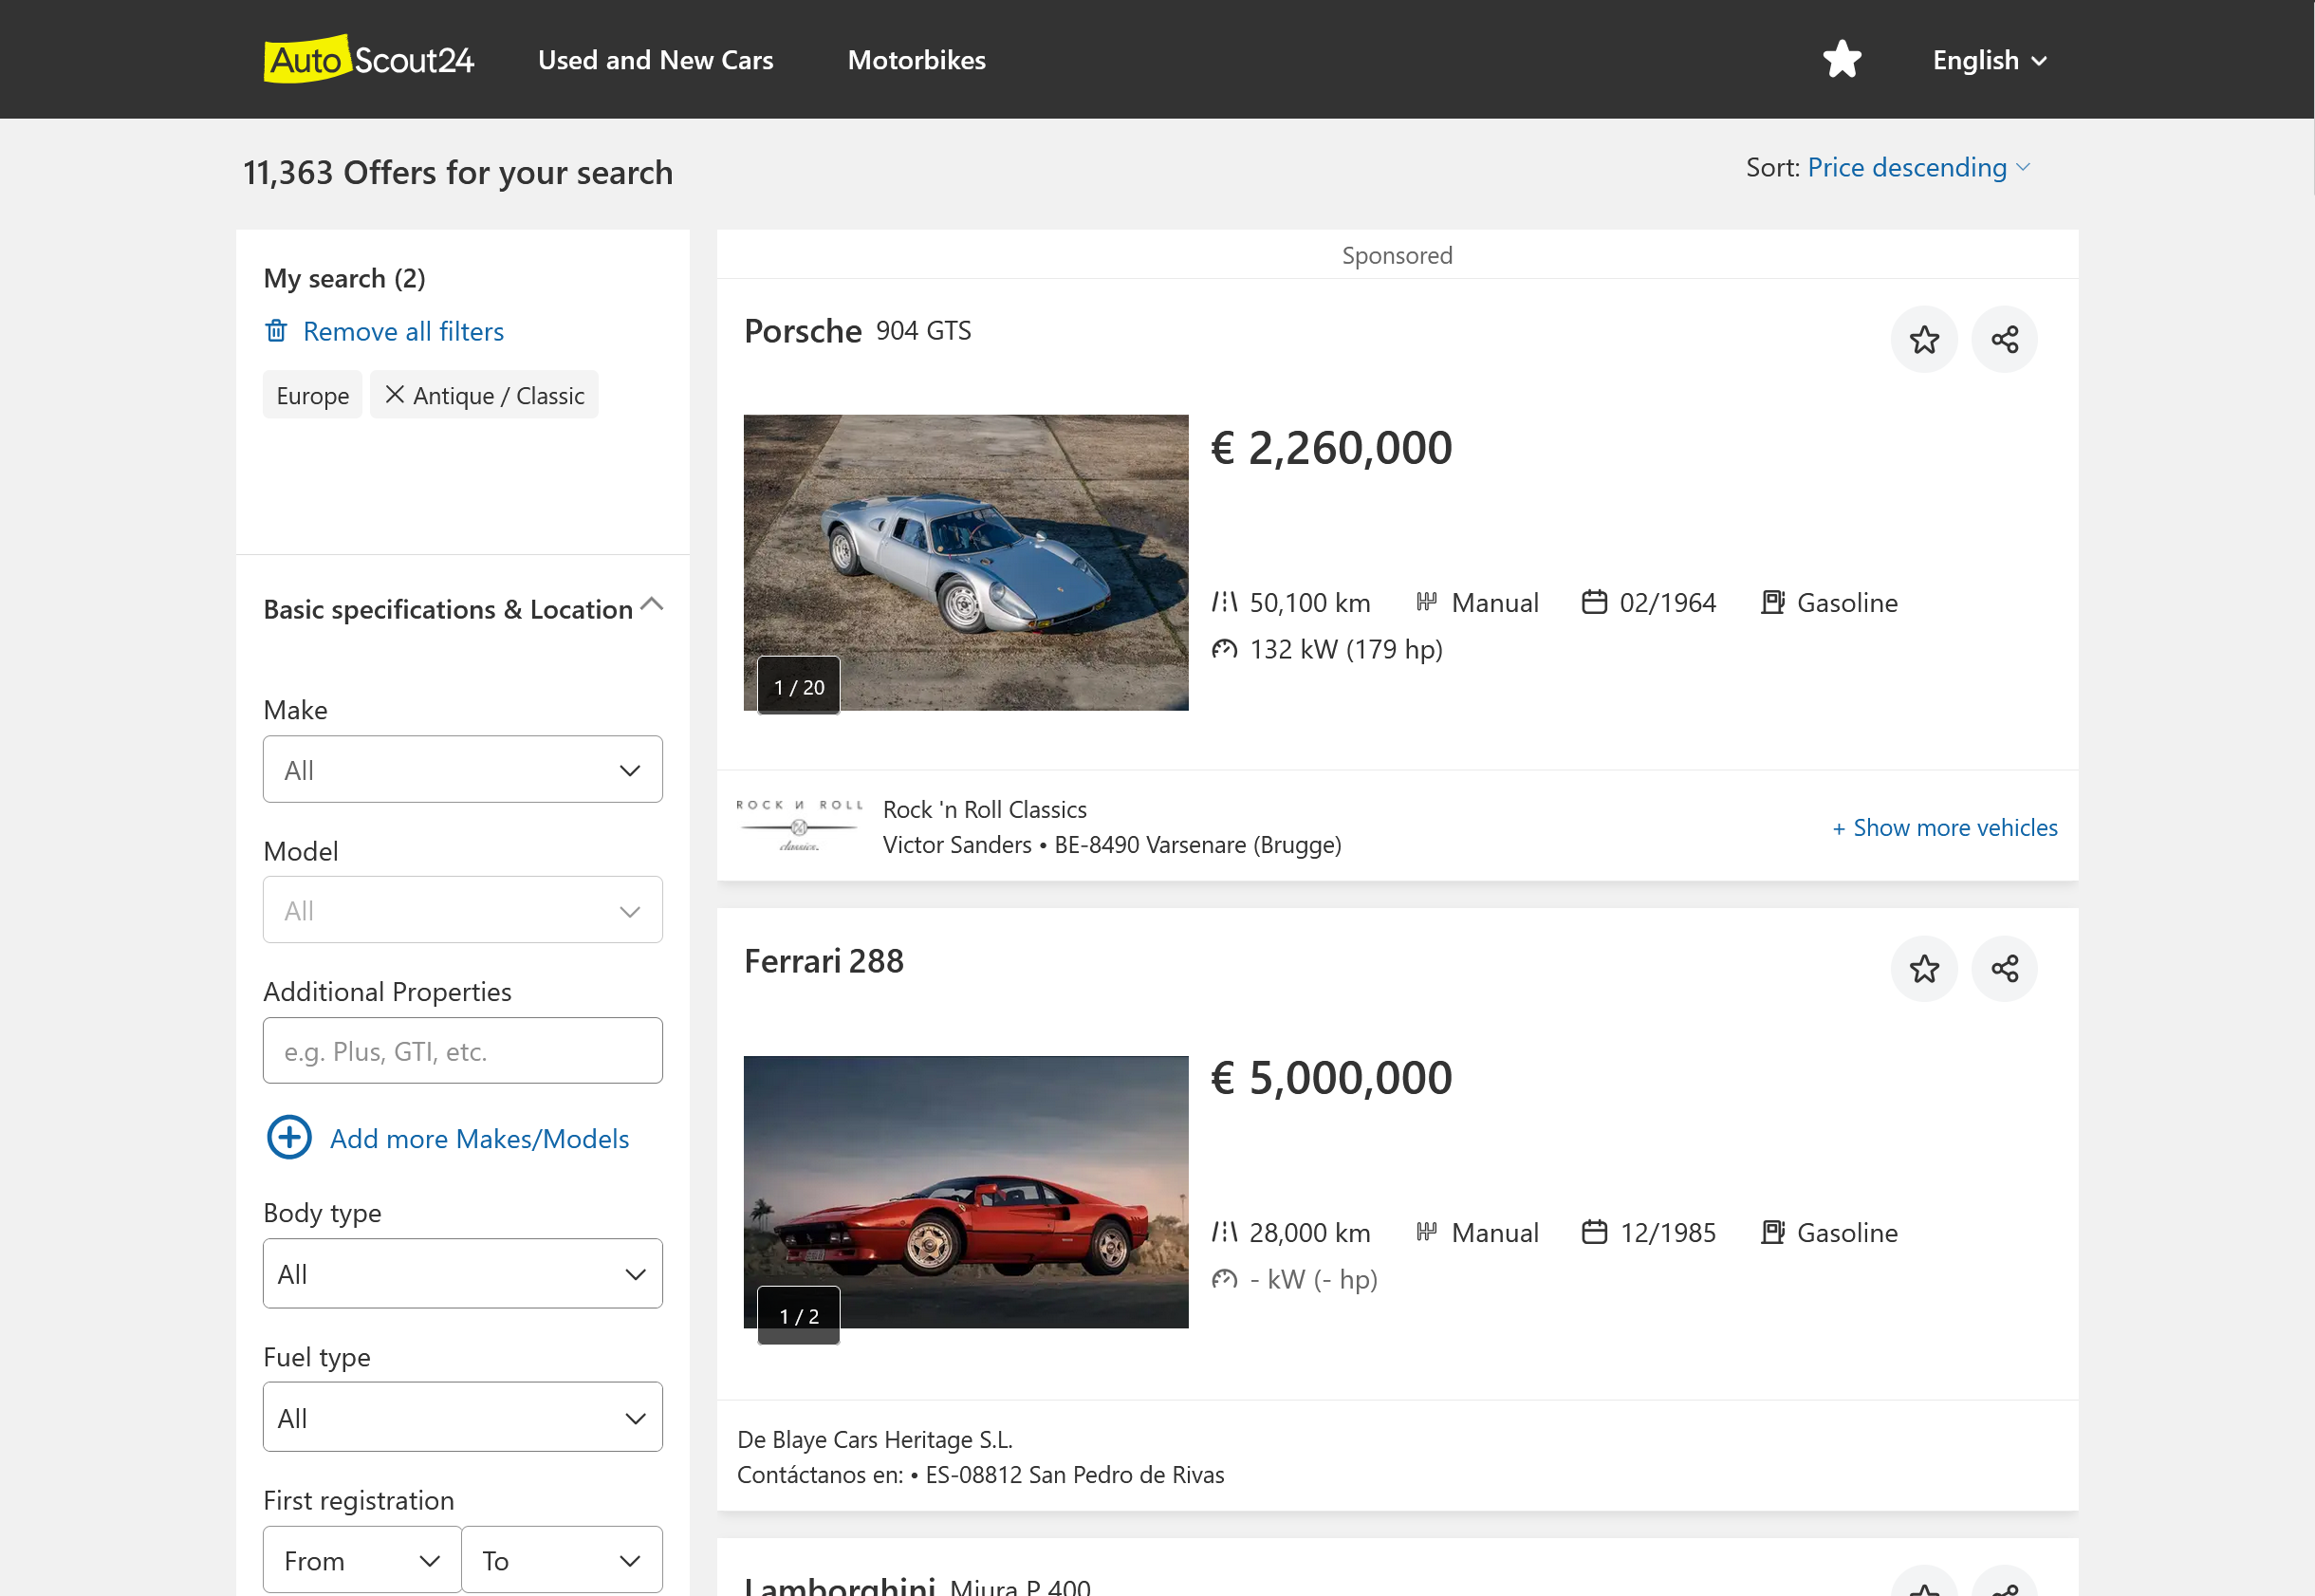
\includegraphics[width=0.8\textwidth]{./images/autoscout.png}
  \caption{Screenshot of Autoscout24 Homepage. source: Autoscout24}
  \label{fig:autoscout}
\end{figure}

The scraping took place from \date{2025-04-03} to \date{2025-04-08}, running practically 24/7 on a laptop even though parallelization was used. In the end we have collected \textit{505804} rows of data, which is a lot more than we could have hoped for in, and wrote it to a \textbf{parquet} file. The scraping consisted of two main parts, which we will discuss in the following subsections along with the bigger challenges we have faced.

\begin{figure}[ht]
  \centering
  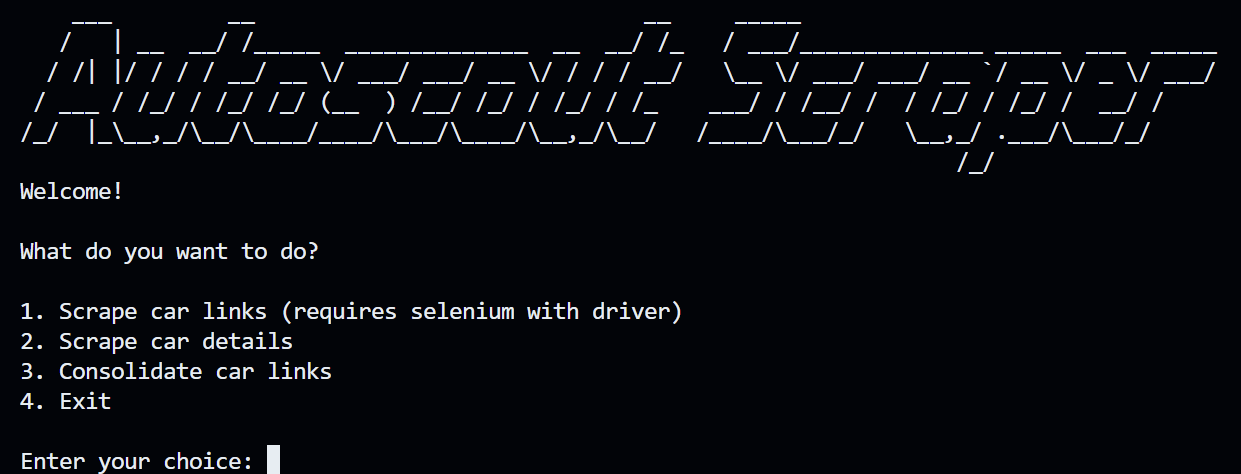
\includegraphics[width=0.8\textwidth]{./images/autoscout_scraper.png}
  \caption{Screenshot of Autoscout Scraper. Source: Autoscout24}
  \label{fig:autoscout_scraper}
\end{figure}

\subsubsection{Scraping Car Listing}

Due to the nature of the website, we needed user interaction for scraping the car listing, so we used \textbf{Selenium} to scrape the URLs pointing to specific car listings. This was achieved through a headless Chromium browser.
We faced two hurdles in this change which we had to overcome with simulated interactions.

\begin{itemize}
  \item \textbf{Pagination:} The website uses a classic pagination system on page, meaning we needed to be able to navigate through each page.
  \item \textbf{Max 20 pages per search:} The website limits the number of returned pages to \textit{20}, so we had to find a way to methodically filter search parameters to find as many sets of \textit{20} pages as possible.
\end{itemize}

In theory almost every common feature of cars can be filtered on the page, so with enough patience one may find all 2 million listings. However, we did not have so much time, nor so many cores on our hands, so we tried finding a middle ground, which was the following:

\begin{enumerate}
  \item Loop through each car make available
  \item For each car make, loop through a range of dynamically changing power ranges in kw based on their presumed likelihood e.g. \texttt{0-15, 15-20, 20-25, 25-26, 26, 27}\dots
  \item For each power range of the car make, loop through the pages available of the pagination
  \item On each pagination page, collect the URLs of the car listings
  \item Store the URLs in a JSON file, keyed by the make
\end{enumerate}

This constituted most of our time scraping, as the user interaction needed to be waited upon and there were simply a lot of possible permutations of make, power, pagination possibilities to go through.
We of course parallelized and worked on multiple cores, also introducing shortcuts, e.g. if we found a make with less than \textit{500} lisitng we did not need to loop through power ranges at all.

\subsubsection{Scraping Car Details}

Once we have collected all the car URLs, the scraping was quite straightforward. We have tested the scraping on individual listings first, trying to find out what categories of data we can scrape and how we may achieve that. At this stage, we were lucky, as no user interaction was needed at all, not even for \textbf{declining cookies}, as the underlying HTML structure already contained the data we needed.
This allowed for us to scrape the data in a much more efficient way, as we could simply use the \textbf{requests} package and \textbf{BeautifulSoup} to parse the HTML and extract the data we needed. This had much lower overhead and allowed us to scrape more listings simultaneously. First fetching into a list in memory, then converting to a df, to then export into a \textbf{parquet} file.

Interesting to note that between the two scraping phases, many links seem to have moved, perhaps due to being sold, or delisted so this case also needed to be addressed.

\subsection{Preprocessing}

We worked separately in numeral Jupyter notebooks, there have been separate notebooks created per each member exploring different aspects of the data. We first started by cleaning the data at the start of each of our own separate notebooks, but later on we decided to do a comprehensive cleaning of the dataset in a separate joint notebook, which can serve as the basis for all of our future work.

The logic can be found in the appropriately named \textbf{data\_cleaning.ipynb} notebook and it contains not only the cleaning logic, but our reasoning behind each of the cleaning steps. We will now summarize the the steps taken in a nutshell.

First off, we got rid of useless features, this included completely empty, almost empty columns and and simply features that we would not need for any of our analysis, like \textbf{manufacturer\_colour} for example.

\begin{figure}[ht]
  \centering
  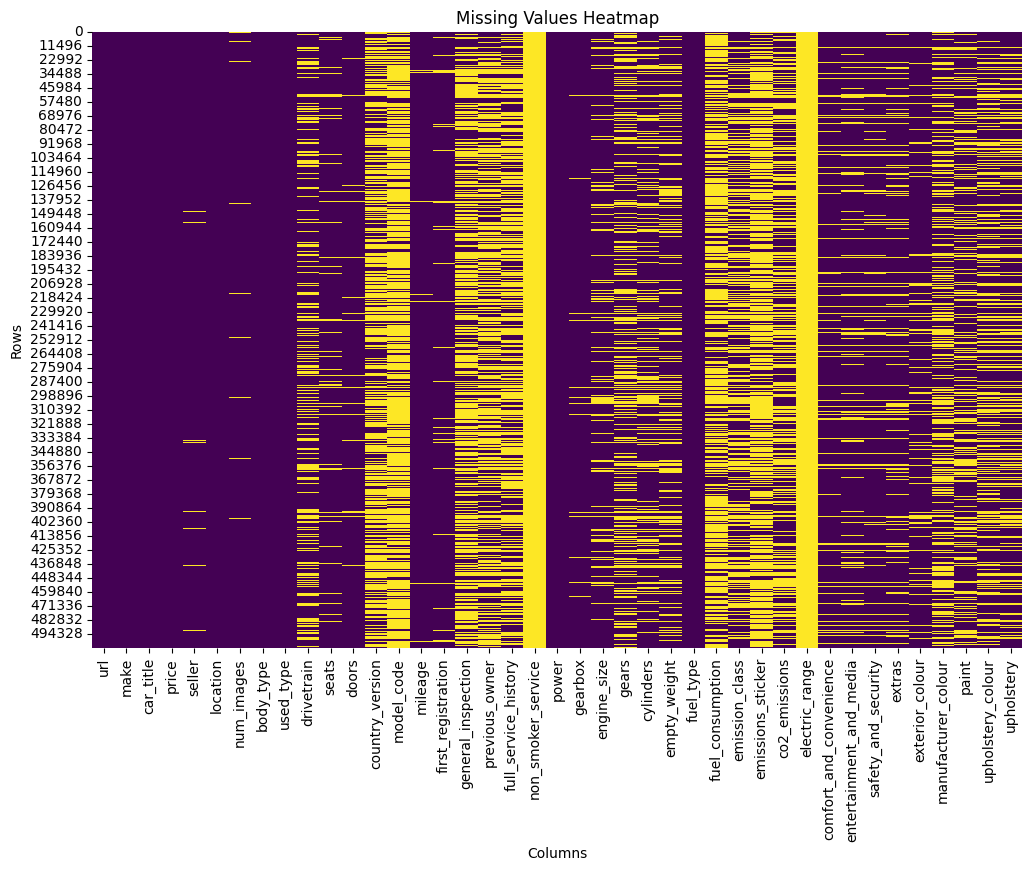
\includegraphics[width=0.8\textwidth]{./images/missing_values_heatmap.png}
  \caption{Missing Values Heatmap. Source: Own work}
  \label{fig:missing_values_heatmap}
\end{figure}

Then, having seen that there are not too many missing values for our main features, \textbf{price}, \textbf{mileage} and \textbf{power}, we decided to drop the rows with missing values, removing \textit{9879} rows, from our 504k large dataset. This seemed like a reasonable choice.

We also had to transform some columns to make them usable for our purposes:

\begin{itemize}
  \item \textbf{Location:} was transformed from the format of \texttt{[city, country code]} to just the country code, as we were not interested in the fine grained location of the car.
  \item \textbf{Fuel consumption:} was similarly transformed from \texttt{[float] l/100 km (comb.)} string format to just the float value.
  \item \textbf{First registration:} was transformed to \textbf{age\_months} by subtracting the first registration date from the current date, as we were only interested in the age of the car, not when it was registered.
\end{itemize}

We found a few imputable / inferable values in our dataset as well:

\begin{itemize}
  \item \textbf{Age:} had seeminlgy \textit{21454} missing values, wehich we could all infer from the column \textbf{use\_type}, whenever this feature was \textbf{New} or \textbf{Demonstration}, we filled the missing values with \textit{0}, as these cars were not used at all. This left us with no missing values at all in this column.
  \item \textbf{Fuel Type:} given that the fuel type was electric, we could safely infer that the \textbf{co2\_emission} was \textbf{0} and that the \textbf{gearbox} was \textbf{automatic}.
\end{itemize}

In the end came the most interesting part, the outlier cleaning. We have inspected 8 of our important numerical features and found that there were some serious outliers in the dataset.

\begin{figure}[ht]
  \centering
  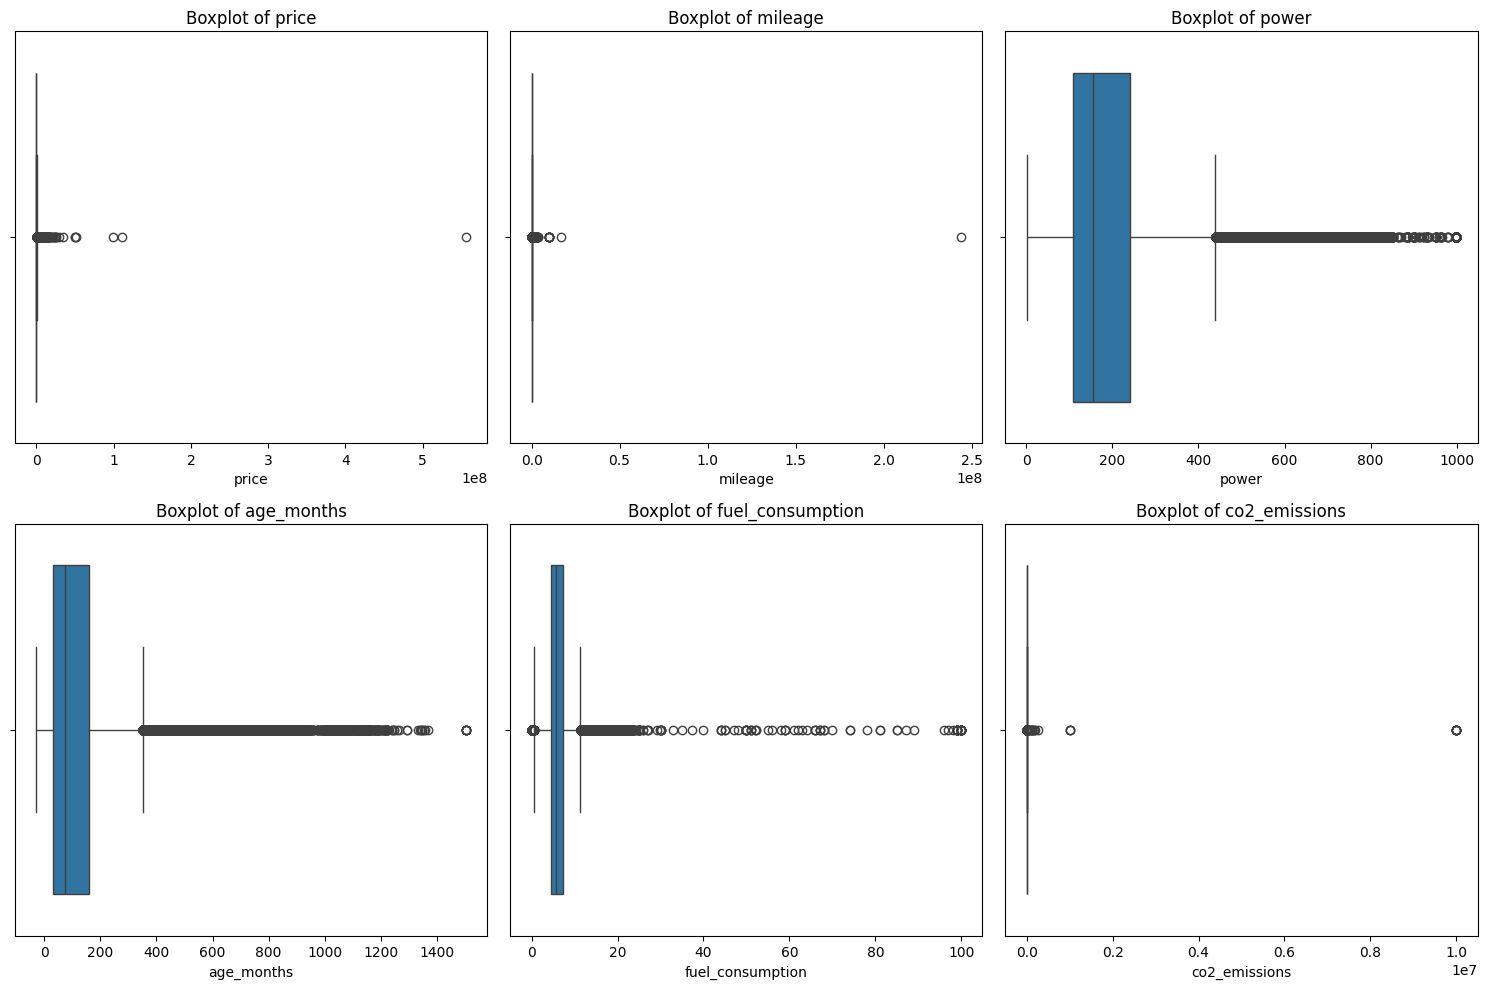
\includegraphics[width=0.8\textwidth]{./images/boxplots_before.png}
  \caption{Boxplots of Numerical Features Before Cleaning. Source: Own work}
  \label{fig:boxplots_before}
\end{figure}

We have used many different strategies to clean the outliers, each based on what felt right for the feature, based on our domain knowledge. Sometimes, we used hard numerical caps, other times used IQR or even 0.05 quantile based capping. As we had so many records to work with, we did not believe winsorization was necessary, so we simply dropped the outliers.
One of the more interesting features to clean was the \textbf{price} as, this had many outliers on both ends and was arguably our most important feature of all. Here we applied a two step process:

\begin{enumerate}
  \item We cleaned the outlers with a lenient 2 * IQR based capping, per car make, as this allowed us to keep values that would have been outliers in the general dataset, but were not outliers at all, e.g. Lamborghini.
  \item Then we manually inspected both ends of the distribution and set a hard cap of \textit{500} EUR on the lower end and \textit{1000000} EUR on the upper end, cleaning out the most extreme outliers. (This inspection led us to notice interesting things, e.g. towable trailers was listed as a car make, which we removed.)
\end{enumerate}

After removing the outliers for other features, with similar care, but less manual inspection, we were left with a much cleaner dataset, as visible from the following boxplots.

\begin{figure}[ht]
  \centering
  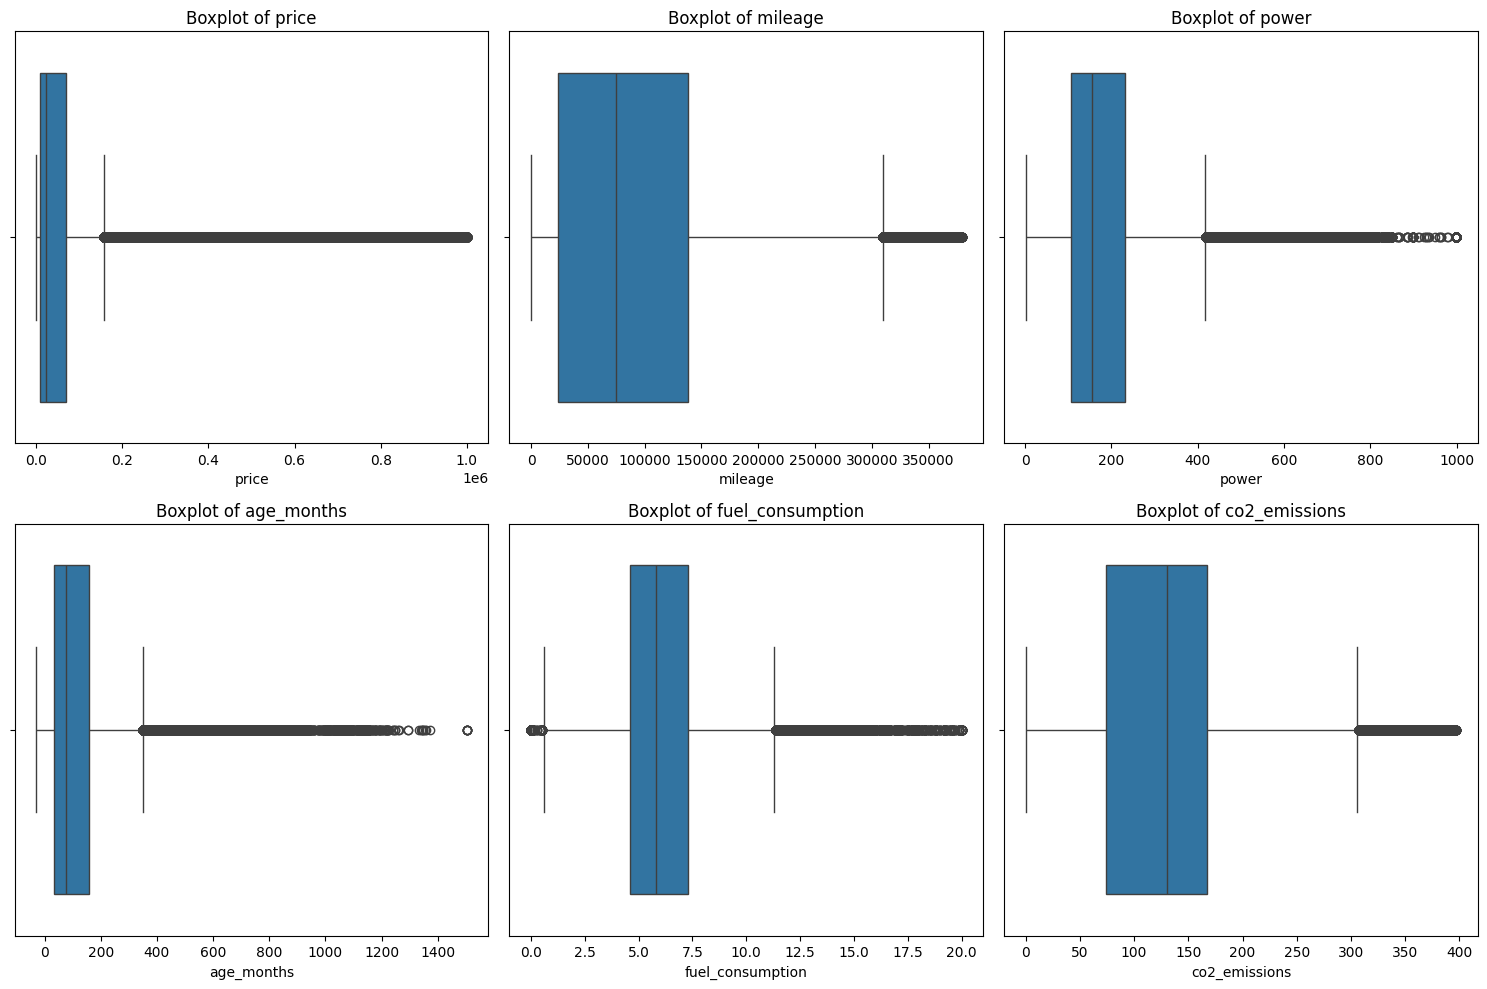
\includegraphics[width=0.8\textwidth]{./images/boxplots_after.png}
  \caption{Boxplots of Numerical Features After Cleaning. Source: Own work}
  \label{fig:boxplots_after}
\end{figure}

The final dataset was then saved to an alternative parquet file, which we will be using for our further analysis. The cleaning here was on purpose not too harsh, such that each subsequent analysis can decide to further clean the data if needed, but we believe we have already found a good balance between keeping the data and cleaning it.
In the end this cleaning process removed \textit{36430} rows from our dataset, which is just \textit{7.2\%} of the original dataset. This seems reasonable, and we have addressed the the possible downsides of our process as losing all the data for some ultra premium car brands, like Koenigsegg, Paganni and losing some data in case a regular car brand happens to have premium models as well, e.g. Nissan GTR.

\subsection{Exploratory Data Analysis}

TODO: Here we will present some interesting findings from our exploratory data analysis.

\subsection{Tools and Software Used}

We used a variety of tools and software for this project, including:

\begin{itemize}
  \item \textbf{Python} primary programming language, used for data scraping, cleaning, and analysis.
  \item \textbf{Selenium} used for web scraping, when user interaction was necessary.
  \item \textbf{BeautifulSoup} for parsing HTML, gathering data from requests.
  \item \textbf{Pandas} for data manipulation and analysis via DataFrames.
  \item \textbf{Matplotlib} and \textbf{Seaborn} for data visualization.
  \item \textbf{Jupyter Notebook} for interactive development and documentation.
  \item \textbf{Scikit-learn} for machine learning and model evaluation.
  \item \textbf{Pytorch} for deep learning models, if applicable.
  \item \textbf{LaTeX} for typesetting and writing the report.
  \item \textbf{Zotero} for managing references and citations.
  \item \textbf{Git} for version control and collaboration between team members.
\end{itemize}

\section{Results}
Describe experiments and the evaluation protocol. Include tables, graphs, and charts as needed to present your findings and results.

\section{Discussion}
Interpret and analyze the results, and discuss possible future work and improvements.

\section{Conclusion}
Provide a summary of the project, key findings, and recommendations. (Approximately 200--350 words.)

\section{Bibliography}

\printbibliography[heading=none]

\section{Self-Reflection}
Add a paragraph or half-page note reflecting on the project.

\end{document}